\documentclass[12pt, twoside,openright]{report}

\usepackage{pdfpages}

\usepackage{setspace}

\usepackage{mathrsfs}

%%%%%%
%The below packages are added by me.
\usepackage{todonotes}
\usepackage{lipsum}  

%%%%%
\usepackage{amsmath,fourier}
\usepackage{mathtools}
\usepackage[no-math]{mathspec}
\setmainfont{Times New Roman} %this sets the main font for the document
\setmathsfont(Digits,Latin,Greek){Times New Roman} % I think you can set individual fonts for different things
%\setmainfont{TeX Gyre Schola} %this sets the main font for the document
%\setmathsfont(Digits,Latin,Greek){TeX Gyre Schola} % I think you can set individual fonts for different things

\usepackage[toc,page]{appendix}

\usepackage{float}
\usepackage{subfigure}
\graphicspath{{Figures/}}
\usepackage{wrapfig}
\usepackage{color}


\usepackage{epigraph}

\setlength\epigraphwidth{\textwidth}


\usepackage{mwe}

\newenvironment{chapterabstract}{%
  \par\nobreak\noindent
  \textbf{\textit{Summary}\hrulefill}\par\nobreak
  \small
  \noindent\ignorespaces
}{%
  \par\nobreak\normalsize
  \vskip-\ht\strutbox\noindent
  \textbf{\hrulefill}%
}

\usepackage[font=small]{caption}

\newcommand*{\mathcolor}{}
\def\mathcolor#1#{\mathcoloraux{#1}}
\newcommand*{\mathcoloraux}[3]{%
  \protect\leavevmode
  \begingroup
    \color#1{#2}#3%
  \endgroup
}


\usepackage[a4paper,bindingoffset=0.2in,left=1in,right=1in,top=1in,bottom=1in,footskip=.25in]{geometry}
%\usepackage{amsmath}
%\usepackage{mathptmx}
%\usepackage[utf8]{inputenc}
\usepackage{graphicx}
\usepackage{multirow}
\usepackage{mathtools}
\usepackage{natbib}




\usepackage{hyperref}



\hypersetup{
    colorlinks=true,
    linkcolor=blue,
    filecolor=magenta,      
    urlcolor=cyan,
citecolor=blue,
 %   pdftitle={Sharelatex Example},
    bookmarks=true,
%    pdfpagemode=FullScreen,
}

\setlength{\arrayrulewidth}{.3mm}
\setlength{\tabcolsep}{18pt}
\renewcommand{\arraystretch}{1.4}
\usepackage[english]{babel}
 
\pagenumbering{roman}
\begin{document}



\begin{titlepage}
    \begin{center}
        \vspace*{1cm}
        \bf 
        LATEX PHD THESIS TEMPLATE OF NITK SURATHKAL

        
        \vspace{0.5cm}
%        Thesis Subtitle
        
        
%        \vfill
 \vspace{3cm}       
        
        Thesis\\
        \vspace{1cm}
        Submitted in partial fulfilment of the requirements for the degree of
        \vspace{1cm}

        DOCTOR OF PHILOSOPHY\\
%IN\\
%PHYSICS

        \vspace{1cm}

    by
    
    \vspace{.5cm}

        \textbf{Firstname Secondname}
        
        \vspace{1cm}
        
        \bf{Reg.No. XXXXXX XXXXXXX}
        
        \vspace{2cm}
   
    
\includegraphics[width=0.2\textwidth]{logo}
  
      
        \vspace{2cm}

        
        
        Department of Physics\\
        NATIONAL INSTITUTE OF TECHNOLOGY KARNATAKA (NITK)\\
        SURATHKAL, MANGALORE - 575 025\\
        \bf{\today} 
        
    \end{center}
\end{titlepage}

\thispagestyle{empty}

\begin{spacing}{1.5}

%%%%%%%%%%%%%%%%%%%%%%%%%%%%%%%%%%%%%%%%%%%%%%%%%%%%%%%%%%%%%%%%%%%%
%Declaration
%%%%%%%%%%%%%%%%%%%%%%%%%%%%%%%%%%%%%%%%%%%%%%%%%%%%%%%%%%%%%%%%%%%%
\newpage
\thispagestyle{empty}
\mbox{}
\newpage
\begin{titlepage}
\begin{center}
\large \textbf{DECLARATION} \\
\textit{By the Ph.D. Research Scholar}
\end{center}

\vspace*{0.5in}
\indent I hereby {\textit{declare}} that the Research Thesis entitled {\bf \textquotedblleft{Thesis Title\textquotedblright}}, which is being submitted to the {\bf\textit{National Institute of Technology Karnataka, Surathkal}} in partial fulfilment of the requirements for the award of the Degree of {\bf\textit{Doctor of Philosophy}} in {\bf\textit{NAME}} is a {\textit{bonafide report of the research work carried out by me}}. The material contained in this thesis has not been submitted to any University or Institution for the award of any degree.

\vspace*{1in}
\begin{singlespacing}
\hspace*{1.5in} 
\parbox{3in}
{\noindent {\bf Firstname Secondname}\\
\noindent {Register No.: XXXXXX XXXXXXX}\\
\noindent {Department of NAME}\\
\noindent {National Institute of Technology Karnataka, Surathkal}}
\end{singlespacing} 

\vspace*{1in}

\noindent Place: NITK, Surathkal\\
\noindent Date: \today 
\end{titlepage}

%%%%%%%%%%%%%%%%%%%%%%%%%%%%%%%%%%%%%%%%%%%%%%%%%%%%%%%%%%%%%%%%%%%
%\clearpage
%\thispagestyle{empty}
%\phantom{a}
%%%%%%%%%%%%%%%%%%%%%%%%%%%%%%%%%%%%%%%%%%%%%%%%%%%%%%%%%%%%%%%%%%%
%Certificate
%%%%%%%%%%%%%%%%%%%%%%%%%%%%%%%%%%%%%%%%%%%%%%%%%%%%%%%%%%%%%%%%%%%
\newpage
\thispagestyle{empty}
\mbox{}
\newpage
\begin{titlepage}
\begin{center}
\large \textbf{CERTIFICATE}
\end{center}

\vspace*{0.5in}
\indent This is to \textit{certify} that the Research Thesis entitled {\bf \textquotedblleft{Thesis Title \textquotedblright}}, submitted by {\bf Firstname Secondname} (Register Number: XXXXXX XXXXXXX) as the record of the research work carried out by him, is \textit{accepted} as the \textit{Research Thesis submission} in partial fulfillment of the requirements for the award of degree of {\bf\textit{Doctor of Philosophy}}.

\vspace*{1in}

\begin{singlespacing}
\hspace*{1.5in} 
\parbox{3in}
{\noindent {\bf Dr FirstName SecondName} \\
\noindent Research Guide \\ 
\noindent Assistant/Associate Professor\\
\noindent Department of NAME\\
\noindent NITK Surathkal - 575025 
\vspace*{1.2in}\\
\noindent {\bf Chairperson - DRPC} \\
\noindent (Signature with Date and Seal)} 
\end{singlespacing} 
\vspace*{0.25in}
\end{titlepage}

%%%%%%%%%%%%%%%%%%%%%%%%%%%%%%%%%%%%%%%%%%%%%%%%%%%%%%%%%%%%%%%%%%%%%
%\clearpage
%\thispagestyle{empty}
%\phantom{a}
%%%%%%%%%%%%%%%%%%%%%%%%%%%%%%%%%%%%%%%%%%%%%%%%%%%%%%%%%%%%%%%%%%%%%

%%%%%%%%%%%%%%%%%%%%%%%%%%%%%%%%%%%%%%%%%%%%%%%%%%%%%%%%%%%%%%%%%%%%%%%%%
%Statements of Contribution
%%%%%%%%%%%%%%%%%%%%%%%%%%%%%%%%%%%%%%%%%%%%%%%%%%%%%%%%%%%%%%%%%%%%%%%%%%
\newpage
\thispagestyle{empty}
\mbox{}
\newpage
\begin{titlepage}
\pagestyle{empty}
\begin{center}
\large \textbf{Statements of Contribution}
\end{center}

%\hspace*{0.5em} \parbox[t]{4.4in}{}
%\vspace*{0.5pt}

\begin{enumerate}
    \item 
   This thesis is based on the following published articles.
\begin{itemize}
    \item Add publication details here
    \item 
    \item
     \item
\end{itemize}
\item
The publications that are not included in the thesis are listed at the end of the thesis under the section titled publications.


\end{enumerate}


\end{titlepage}


%%%%%%%%%%%%%%%%%%%%%%%%%%%%%%%%%%%%%%%%%%%%%%%%%%%%%%%%%%%%%%%%%%%%
%\clearpage
%\thispagestyle{empty}
%\phantom{a}
%%%%%%%%%%%%%%%%%%%%%%%%%%%%%%%%%%%%%%%%%%%%%%%%%%%%%%%%%%%%%%%%%%%%%


%%%%%%%%%%%%%%%%%%%%%%%%%%%%%%%%%%%%%%%%%%%%%%%%%%%%%%%%%%%%%%%%%%%%%%%%%
%Abstract
%%%%%%%%%%%%%%%%%%%%%%%%%%%%%%%%%%%%%%%%%%%%%%%%%%%%%%%%%%%%%%%%%%%%%%%%%%
\newpage
\thispagestyle{empty}
\mbox{}
\newpage
\begin{titlepage}
\pagestyle{empty}
\begin{center}
\large \textbf{ABSTRACT}
\end{center}

%\hspace*{0.5em} \parbox[t]{4.4in}{}
%\vspace*{0.5pt}

\hspace*{0cm}
\lipsum[1]
\lipsum[2]

\vspace*{12pt}
\noindent \textit {Keywords}: {Energy, Matter, Publications, PhD, Job}




\end{titlepage}


%%%%%%%%%%%%%%%%%%%%%%%%%%%%%%%%%%%%%%%%%%%%%%%%%%%%%%%%%%%%%%%%%%%%
%\clearpage
%\thispagestyle{empty}
%\phantom{a}
%%%%%%%%%%%%%%%%%%%%%%%%%%%%%%%%%%%%%%%%%%%%%%%%%%%%%%%%%%%%%%%%%%%%%


%%%%%%%%%%%%%%%%%%%%%%%%%%%%%%%%%%%%%%%%%%%%%%%%%%%%%%%%%%%%%%%%%%%%%%%%%
%Acknowledgements
%%%%%%%%%%%%%%%%%%%%%%%%%%%%%%%%%%%%%%%%%%%%%%%%%%%%%%%%%%%%%%%%%%%%%%%%%%
\newpage
\thispagestyle{empty}
\mbox{}
\newpage
\begin{titlepage}
\pagestyle{empty}
\begin{center}
\large \textbf{Acknowledgements}
\end{center}


%\hspace*{0.5em} \parbox[t]{4.4in}{}
%\vspace*{0.5pt}

\hspace*{0cm}

\lipsum[1]
\lipsum[2]


\end{titlepage}


%%%%%%%%%%%%%%%%%%%%%%%%%%%%%%%%%%%%%%%%%%%%%%%%%%%%%%%%%%%%%%%%%%%%
%\clearpage
%\thispagestyle{empty}
%\phantom{a}
%%%%%%%%%%%%%%%%%%%%%%%%%%%%%%%%%%%%%%%%%%%%%%%%%%%%%%%%%%%%%%%%%%%%%


%%%%%%%%%%%%%%%%%%%%%%%%%%%%%%%%%%%%%%%%%%%%%%%%%%%%%%%%%%%%%%%%%%%%%%%%%
%Dedication
%%%%%%%%%%%%%%%%%%%%%%%%%%%%%%%%%%%%%%%%%%%%%%%%%%%%%%%%%%%%%%%%%%%%%%%%%%
%\newpage
%\thispagestyle{empty}
%\mbox{}
\newpage
\begin{titlepage}
\pagestyle{empty}
\begin{center}
\large \textbf{Dedication}
\end{center}

\hspace*{0.5em} \parbox[t]{4.4in}{}
\vspace*{0.5pt}

\hspace*{0cm}

\begin{center}
\emph{ Write the dedication here.}
\end{center}



\end{titlepage}


%%%%%%%%%%%%%%%%%%%%%%%%%%%%%%%%%%%%%%%%%%%%%%%%%%%%%%%%%%%%%%%%%%%%
%\clearpage
%\thispagestyle{empty}
%\phantom{a}
%%%%%%%%%%%%%%%%%%%%%%%%%%%%%%%%%%%%%%%%%%%%%%%%%%%%%%%%%%%%%%%%%%%%%

\newpage
\tableofcontents
\listoffigures
\addcontentsline{toc}{chapter}{List of figures}

\listoftables
\addcontentsline{toc}{chapter}{List of tables}

\chapter{Introduction}
\label{Introduction_Chapter}
\pagenumbering{arabic}
\setcounter{page}{1}

% The epigraph is optional. If you do not like it, comment it out.

\epigraph{If I have seen further, it is by standing on the shoulders of giants.}{Isaac Newton}

% Write a brief summary of the chapter here.

\begin{chapterabstract}
This chapter gives a basic introduction to LATEX. For more, visit \url{https://www.overleaf.com/learn/latex/Learn_LaTeX_in_30_minutes}
\end{chapterabstract}


LATEX (pronounced LAY-tek or LAH-tek) is a tool used to create professional-looking documents. It is based on the WYSIWYM (what you see is what you mean) idea, meaning you only have focus on the contents of your document and the computer will take care of the formatting. Instead of spacing out text on a page to control formatting, as with Microsoft Word or LibreOffice Writer, users can enter plain text and let LATEX take care of the rest.

LATEX is used all over the world for scientific documents, books, as well as many other forms of publishing. Not only can it create beautifully typeset documents, but it allows users to very quickly tackle the more complicated parts of typesetting, such as inputting mathematics, creating tables of contents, referencing and creating bibliographies, and having a consistent layout across all sections. Due to the huge number of open source packages available (more on this later), the possibilities with LATEX are endless. These packages allow users to do even more with LATEX, such as add footnotes, draw schematics, create tables etc.

One of the most important reasons people use LATEX is that it separates the content of the document from the style. This means that once you have written the content of your document, we can change its appearance with ease. Similarly, you can create one style of document which can be used to standardise the appearance of many different documents. This allows scientific journals to create templates for submissions. These templates have a pre-made layout meaning that only the content needs to be added. In fact there are hundreds of templates available for everything from CVs to slideshows.


\section{Objectives of the Thesis}
\lipsum[1-2] 

% Make a bullets list 

\begin{itemize}

\item 
\lipsum[1]

\item
\lipsum[2]

\item 
\lipsum[3]

\item
\lipsum[4]

\end{itemize}

\section{Organisation of the Thesis}

% Write a brief chapterwise organisation of the thesis here.

The thesis is organised as follows:

{\bf Chapter 1}: This chapter gives a brief introduction to the thesis.
\lipsum[1]


{\bf Chapter 2}: \lipsum[2] 

{\bf Chapter 3}: The thesis is summarised here with a discussion on results and future research.
%%%%%%%%%%%%%%%%%%%%%%%%%%%%%%%%%%%%%%%%%%%%%%%%%%%%%%%%%%%%%%%%%%%%
%%%%%%%%%%%%%%%%%%%%%%%%%%%%%%%%%%%%%%%%%%%%%%%%%%%%%%%%%%%%%%%%%%%%%%%%%%%%%%%%%%%%%%%%%%%%%%%%%


\chapter{Title of the chapter}
%%%%%%%%%%%%%%%%%%%%%%%%%%%%%%%%%%%%%%%%%%%%%%%%%%%%%%%%%%%%%%%%%%%%%%%%%%%%%%%%%%%%%%%%%%%%%%%%%%%%%%%%%%%%%%%%%%%%%%%%%%%%%%%%%%%%%%%%%%%%%%%%%%%%%%%%%%%
\epigraph{If I have seen further, it is by standing on the shoulders of giants.}{Isaac Newton}
\begin{chapterabstract}
Lorem Ipsum is simply dummy text of the printing and typesetting industry. Lorem Ipsum has been the industry's standard dummy text ever since the 1500s, when an unknown printer took a galley of type and scrambled it to make a type specimen book. It has survived not only five centuries, but also the leap into electronic typesetting, remaining essentially unchanged. It was popularised in the 1960s with the release of Letraset sheets containing Lorem Ipsum passages, and more recently with desktop publishing software like Aldus PageMaker including versions of Lorem Ipsum.
\end{chapterabstract}
% The following text is taken from wikipedia page https://en.wikipedia.org/wiki/Physics#/media/File:Stylised_atom_with_three_Bohr_model_orbits_and_stylised_nucleus.png

Physics is the natural science that studies matter \citep{Poisson:2009pwt} its fundamental constituents, its motion and behavior through space and time, and the related entities of energy and force. Physics is one of the most fundamental scientific disciplines, and its main goal is to understand how the universe behaves.

This is how you cite \citep{Abbott:2016blz}.  

To write a equation do the following:

\begin{equation}
\{ u_t(x,t)=u_{xx}(x,t)\}, \text{ where $\epsilon\in\mathbb{R}$ and $t>0$}
\label{eq:heat_equation}
\end{equation}

This is how you cite a equation \ref{eq:heat_equation}, chapter \ref{Introduction_Chapter} or a figure \ref{fig:Bohr_Model}.




\begin{figure}
    \centering
    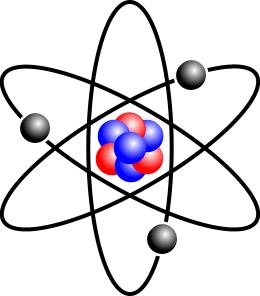
\includegraphics[width=\textwidth, height=11cm]{Bohr_Model.png}
    \caption{Bohr Model of an atom.}
    \label{fig:Bohr_Model}
\end{figure}










%%%%%%%%%%%%%%%%%%%%%%%%%%%%%%%%%%%%%%%%%%%%%%%%%%%%%%%%%%%%%%%%%%%%%%%%%%%%%%%%%%%%%%%%%%%%%%%%%%%%%%%%%%%%%%%%%%%%%%%%%%%%%%%%%%%%%%%%%%%%%%%%%%%%%%%%%%%



\chapter{Conclusion}

\epigraph{Stay hungry stay foolish.}{Steve Jobs, \textit{originally took from the Whole Earth Catalog (1974)}}



\section{Conclusions}

\section{Future Directions}


%%%%%%%%%%%%%%%%%%%%%%%%%%%%%%%%%%%%%%%%%%%%%%%%%%%%%%%%%%%%%%%%%%%%%%%%%%%%%%%%%%%%%%%%%%%%%%%%%%%%%%%%%%%%%%%%%%%%%
\chapter*{Appendix}
\addcontentsline{toc}{chapter}{Appendix}

\section*{Title here}






\end{spacing} 





\bibliographystyle{apalike}
\addcontentsline{toc}{section}{References}
\bibliography{mybib}


%%%%%%%%%%%%%%%%%%%%%%%%%%%%%%%%%%%%%%%%%%%%%%%%%%%%%%%%%%%%%%%%%%%%%%%%%%%%%%%%%%%%%%%%%%%%%%%%%%%%%%%%%%%%%%%%%%%%%

\chapter*{List of publications}
\addcontentsline{toc}{section}{List of publications}

\section*{Peer Reviewed International Journals}
\begin{itemize}
   
    \item
    Shreyas Punacha, {\bf Naveena Kumara A.}, and T. K. Shajahan,  "Theory of unpinning of spiral waves using circularly polarized electric fields in mathematical models of excitable media", \emph{Physical Review E 102, 032411 (2020)}
    \end{itemize}
    
   \section*{arXiv Pre-prints} 
   \begin{itemize}
   \item
\end{itemize}

\section*{Peer Reviewed International Journal proceedings}
\begin{itemize}
    \item
\end{itemize}

\section*{International Conferences Presentations}
\begin{itemize}
    \item  
\end{itemize}


\newpage
\thispagestyle{empty}
\mbox{}


\newpage
\clearpage
\thispagestyle{empty}
\phantom{a}


\begin{center}
\large \underline{\textbf{CURRICULUM VITAE}}
\end{center}
%\addcontentsline{toc}{chapter}{Curriculum Vitae}
\vspace*{0.1in}

%%%%%%%%%%%%%%%%%%%%%%%%%%%%%%%%%%%

\end{document}
